\section{Parte A}

        \textbf{1) De que forma as perdas e duplicações de pacotes afetaram o desempenho das aplicações? Que camada lidou com as perdas e duplicações: transporte ou aplicação? Responda com base nas experiências feitas e nos resultados observados.}

        As perdas e duplicações de pacotes afetam diretamente o funcionamento da rede, o que por sua vez causa sérios prejuízos no desempenho das aplicações.
        
        No caso da perda de pacotes, os tempos de espera efetuados pelos \textit{end systems} tendem a aumentar, visto que em princípio é necessária a retransmissão desses mesmos pacotes. Já na situação da duplicação de vários pacotes, a rede corre o risco de ficar congestionada, contribuindo assim para uma transferência de informação mais vagarosa entre múltiplos \textit{end systems.}

        Os \textit{layers} $4$ e $5$ estão preparados para lidar com estas situações, contudo, dependendo do protocolo utilizado na camada de transporte, essa responsabilidade recai sobre um determinado \textit{layer.}

        Caso o TPC seja o protocolo utilizado, é a camada de transporte que resolve os problemas, visto que é assegurada uma comunicação fiável, capaz de garantir o controlo de congestão, fluxo e erros.

        \begin{itemize}
            \item \textbf{Pacotes perdidos:} A partir do momento em que um \textit{acknowledgement} não é recebido, a camada de transporte pede uma retransmissão do pacote perdido, sem que o nível aplicacional perceba.
            \item \textbf{Pacotes duplicados:} Ao serem identificados pacotes com o mesmo valor de \textit{Seq} e \textit{Ack,} a camada de transporte percebe de imediato que se tratam de pacotes duplicados e portanto opta por ignorá-los.
        \end{itemize}

        Relativamente ao UDP, a situação é completamente diferente, pois não havendo uma transmissão fiável, apenas existe a preocupação de enviar pacotes independentemente do estado da rede e da existência de um \textit{end system} que esteja disposto a receber essa informação.

        \begin{itemize}
            \item \textbf{Pacotes perdidos:} O UDP não faz uso dos \textit{acknowledgements,} como tal é a camada aplicacional que deteta os pacotes perdidos e pede a retransmissão dos mesmos.
            \item \textbf{Pacotes duplicados:} O UDP não possui a capacidade de identificar pacotes duplicados, portanto a camada aplicacional procura fazer uma filtragem da informação e descartar aquilo que seja redundante.
        \end{itemize}

        \begin{figure}[hb!]
            \centering
            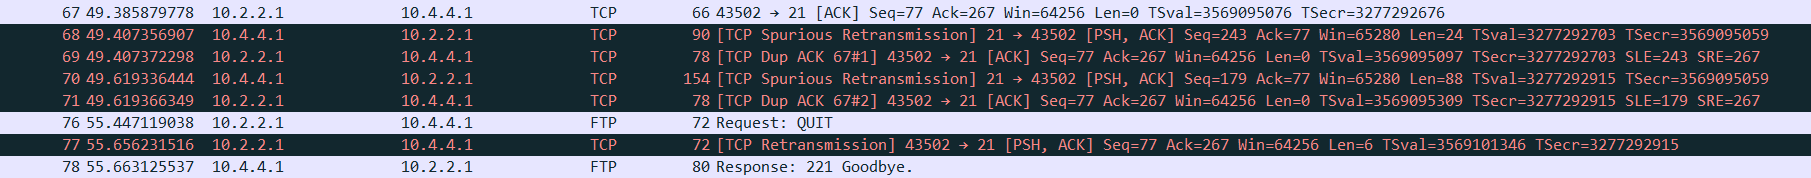
\includegraphics[width=\textwidth]{Imagens/1.png}
            \caption{Captura da comunicação FTP entre o \textit{PC1} e o \textit{Servidor1}}
            \vspace{-10pt}
        \end{figure}

        Como podemos ver pela captura apresentada, foi o TCP (protocolo da camada de transporte) que identificou os pacotes duplicado e além disso solicitou a retransmissão daqueles que se tinham perdido.

        \begin{figure}[hb!]
            \centering
            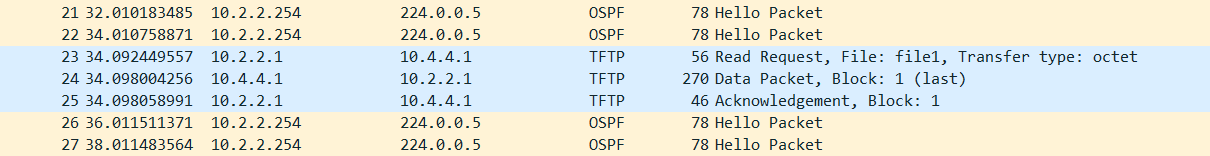
\includegraphics[width=\textwidth]{Imagens/2.png}
            \caption{Captura da comunicação TFTP entre o \textit{PC1} e o \textit{Servidor1}}
            \vspace{-10pt}
        \end{figure}

        Em relação ao comportamento da camada aplicacional, não tivemos a oportunidade de ver aquilo que depreendemos, visto que não ocorreu qualquer perda ou duplicação de pacotes.

        \textbf{2) Obtenha a partir do \textit{Wireshark,} ou desenhe manualmente, um diagrama temporal para a transferência de \textit{file1} por FTP. Foque-se apenas na transferência de dados [ftp-data] e não na conexão de controlo, pois o FTP usa mais que uma conexão em simultâneo. Identifique, se aplicável, as fases de início de conexão, transferência de dados e fim de conexão. Identifique também os tipos de segmentos trocados e os números de sequência usados quer nos dados como nas confirmações.}

        Dado que o FTP utiliza o TCP como protocolo da camada de transporte, e apenas pretendemos analisar a transferência de dados [ftp-data], optámos por aplicar o filtro \textit{tcp.port == 20.}

        \begin{figure}[hb!]
            \centering
            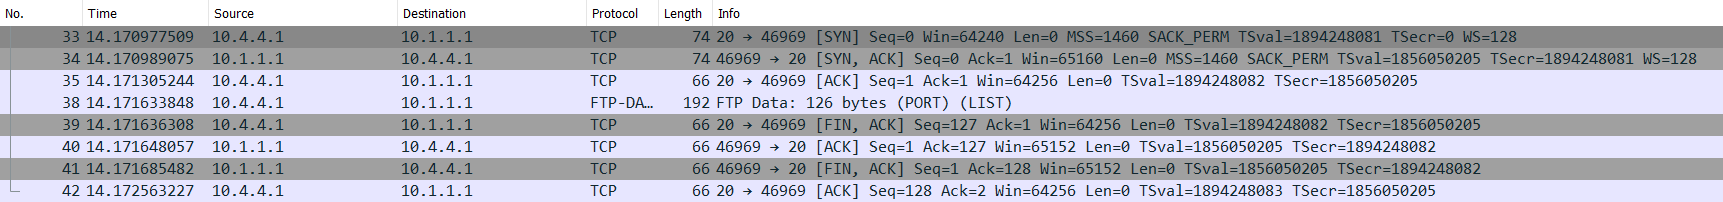
\includegraphics[width=\textwidth]{Imagens/3.png}
            \caption{Captura da comunicação FTP entre o \textit{Portatil1} e o \textit{Servidor1}}
            \vspace{-10pt}
        \end{figure}

        \newpage

        \begin{figure}[hb!]
            \centering
            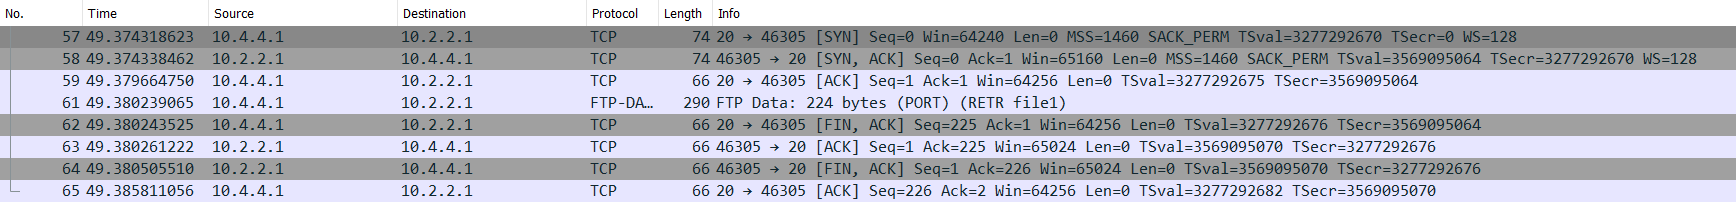
\includegraphics[width=\textwidth]{Imagens/4.png}
            \caption{Captura da comunicação FTP entre o \textit{PC1} e o \textit{Servidor1}}
            \vspace{-10pt}
        \end{figure}

        As duas capturas são praticamente iguais, exceptuando o facto do endereço IP associado aos \textit{end systems,} todavia optámos por traçar um diagrama temporal para cada uma das transferência de \textit{file1} por FTP. 

        \begin{figure}[hb!]
            \centering
            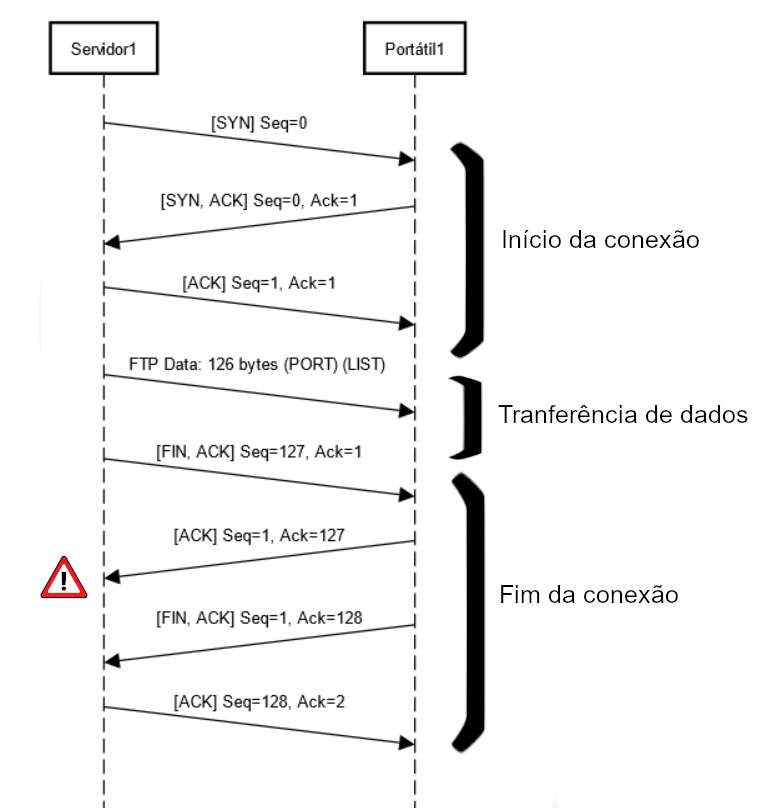
\includegraphics[width=0.6\textwidth]{Imagens/5.png}
            \caption{Diagrama temporal da comunicação FTP entre o \textit{Portatil1} e o \textit{Servidor1}}
            \vspace{-10pt}
        \end{figure}

        Sendo o TCP um protocolo orientado à conexão, é necessário estabelecer e reservar um canal lógico para efetuar a transferência de segmentos, o que por sua vez implica uma fase de início da conexão, transferência de dados e fim da conexão.

        Durante as fases de início e fim da conexão, os \textit{acknowledgements} possuem um $Acknum = x+1$, sendo que $x$ é o número de sequência da mensagem que pretendemos confirmar. Em relação à transferência de dados não se verifica a mesma situação, uma vez que $Acknum = x + y$, onde $x$ é o número de sequência e $y$ os \textit{bytes} transferidos pela mensagem que se pretende confirmar.

        Há que ter em atenção que o segmento identificado com o sinal de perigo é referente à transferência de dados, apesar de estar posicionado na secção de fim da conexão. Tal aconteceu porque o \textit{Servidor1} enviou o segmento [FIN, ACK] antes do \textit{Portatil1} enviar o \textit{acknowledgement} a dizer que tinha recebido corretamente os dados.
        
        Talvez isto tenha acontecido, porque o \textit{Servidor1} já "sabia"~que não teria de enviar mais nada, e portanto decidiu tomar a iniciativa de terminar a conexão com o \textit{Portatil1}, enviando por isso o segmento [FIN, ACK].

        Além disso, verificámos que esta situação também se registou na outra captura, pelo que depreendemos que este comportamento seja típico do \textit{Servidor1.} O que de certo modo faz sentido, visto que o único objetivo das comunicações efetuadas era pura e simplesmente transferir o arquivo \textit{file1.}

        \begin{figure}[hb!]
            \centering
            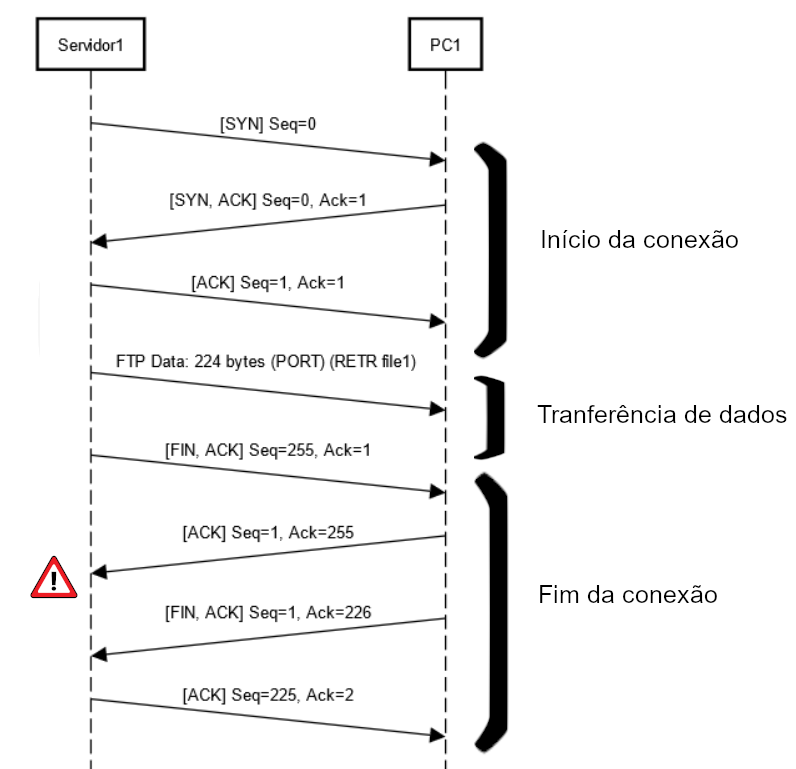
\includegraphics[width=0.6\textwidth]{Imagens/6.png}
            \caption{Diagrama temporal da comunicação FTP entre o \textit{PC1} e o \textit{Servidor1}}
            \vspace{-10pt}
        \end{figure}

        \textbf{3) Obtenha a partir do \textit{Wireshark,} ou desenhe manualmente, um diagrama temporal para a transferência de file1 por TFTP. Identifique, se aplicável, as fases de início de conexão, transferência de dados e fim de conexão. Identifique também os tipos de segmentos trocados e os números de sequência usados quer nos dados como nas confirmações.}

        Ao analisar as capturas tanto do \textit{end system} \textit{Portatil1} com  de \textit{PC1,} percebemos claramente que estas são bastante semelhantes, alterando-se apenas o endereço IP associado a cada um dos dispositivos.

        \newpage
        \begin{figure}[hb!]
            \centering
            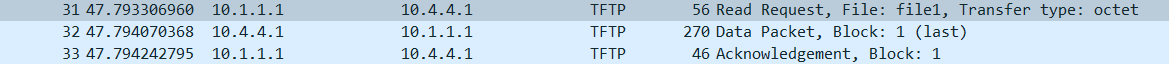
\includegraphics[width=\textwidth]{Imagens/7.png}
            \caption{Captura da comunicação TFTP entre \textit{Portatil1} e \textit{Servidor1}}
            \vspace{-10pt}
        \end{figure}

        \begin{figure}[hb!]
            \centering
            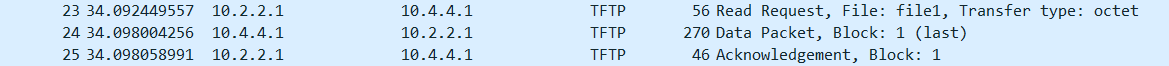
\includegraphics[width=\textwidth]{Imagens/8.png}
            \caption{Captura da comunicação TFTP entre \textit{PC1} e \textit{Servidor1}}
            \vspace{-10pt}
        \end{figure}

        O facto de não termos obtido nenhuma retransmissão na segunda captura deixou-nos um pouco perplexos, visto que o TFTP utiliza como protocolo de transporte o UDP (não fiável), além disso o canal entre a \textit{Local Network 2} e o \textit{Core} tem um \textit{throughput} baixo e uma perda percentual bastante elevada, o que propícia a perda de pacotes.

        \begin{figure}
            \vspace{-10pt}
             \centering
             \begin{subfigure}[b]{0.4\textwidth}
                 \centering
                 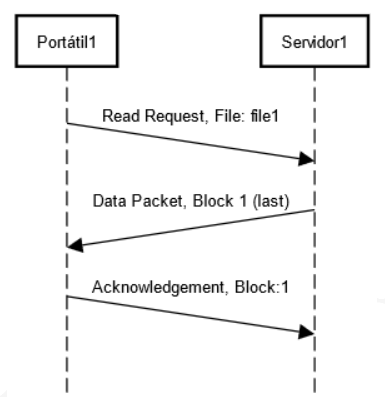
\includegraphics[width=\textwidth]{Imagens/9.png}
                 \caption*{Comunicação TFTP entre \textit{Portatil1} e \textit{Servidor1}}
             \end{subfigure}
             \hfill
             \begin{subfigure}[b]{0.4\textwidth}
                 \centering
                 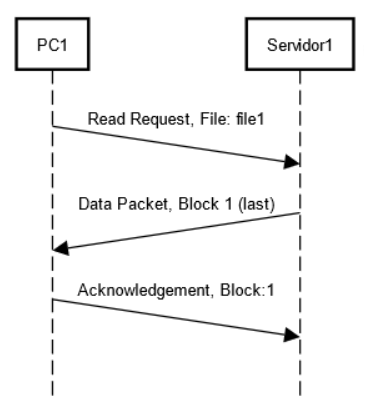
\includegraphics[width=\textwidth]{Imagens/10.png}
                 \caption*{Comunicação TFTP entre \textit{PC1} e \textit{Servidor1}}
             \end{subfigure}
             \caption{Diagrama temporal das comunicações TFTP}
             \vspace{-10pt}
        \end{figure}

        O UDP é um protocolo da camada de transporte não orientado à conexão, como tal um \textit{socket} UDP está sempre preparado a enviar/receber dados, tendo isto em mente, concluímos que nem sequer é estabelecida uma ligação formal antes do envio de dados, pelo que não existem as fases de início e fim da conexão.

        \begin{itemize}
            \item \textbf{1º segmento:} O  cliente TFTP efetua um pedido de leitura ao servidor.

            \item \textbf{2º segmento:} O cliente e o servidor realizam a troca de dados solicitados pelo segmento anterior.

            \item \textbf{3º segmento} Quando a transmissão de dados termina, o cliente confirma a receção dos mesmos.
        \end{itemize}

        Sendo que o UDP não faz uso de \textit{acknowledgements,} o terceiro segmento pode parecer um pouco suspeito, contudo reflete apenas o facto de o TFTP estar a assumir funções que seriam normalmente asseguradas pelo TCP, ou seja, a confirmação da receção dos segmentos, tendo em vista a sua retransmissão caso haja essa necessidade.

        \textbf{4) Compare sucintamente as quatro aplicações de transferência de ficheiros que usou nos seguintes pontos (i) uso da camada de transporte; (ii) eficiência; (iii) complexidade; (iv) segurança}

        \vspace{5pt}
        \textbf{\large SFTP}
        
        \begin{itemize}
            
            \item \textbf{Protocolo de transporte:} TCP \textit{(Transmission Control Protocol).} 
            
            \item \textbf{Eficiência:} Possui muito \textit{overhead} resultante da criação de chaves, quer para a encriptação e desencriptação de dados, quer para a autenticação do cliente ao servidor.  
            
            \item \textbf{Complexidade:} A utilização chaves SSH como forma de autenticação e encriptação, demonstra um certo nível de complexidade, o que por sua vez atrasa a transferência de dados.
            
            \item \textbf{Segurança:} A emprego dos pares chave pública/privada na fase de autenticação, bem como na encriptação, torna a conexão extremamente segura.
        
        \end{itemize}

        \textbf{\large FTP}
        \begin{itemize}
            
            \item \textbf{Protocolo de transporte:} TCP \textit{(Transmission Control Protocol).} 
            
            \item \textbf{Eficiência:} Como utiliza o TCP, tende a gerar algum \textit{overhead} por via do cabeçalho, além disso as implicações deste protocolo (controlo de congestão/fluxo/erros) costumam atrasar a transferência de dados. 
            
            \item \textbf{Complexidade:} Mesmo possuindo uma fase de autenticação e diferentes modos de transferência de dados, é bastante simplista, visto que baseia-se essencialmente na transferência de ficheiros.
            
            \item \textbf{Segurança:} Apesar de possibilitar a criação de vários utilizadores com as respetivas \textit{passwords,} a conexão em si é bastante insegura.
        
        \end{itemize}

        \textbf{\large TFTP}
        \begin{itemize}
            
            \item \textbf{Protocolo de transporte:} UDP \textit{(User Datagram Protocol).}
            
            \item \textbf{Eficiência:} A utilização do UDP contribui para um menor \textit{overhead} dos cabeçalhos, além disso a transferência de dados é mais rápida, uma vez que não há controlo de erros por parte da camada de transporte.
            
            \item \textbf{Complexidade:} Como é aplicado somente na transferência de ficheiros e não possui quaisquer métodos de segurança, acaba por revelar-se extremamente simplista.
            
            \item \textbf{Segurança:} Revela uma enorme falta de segurança, dada a ausência de quaisquer métodos de autenticação ou encriptação de dados.

        \end{itemize}

        \textbf{\large HTTP}
        \begin{itemize}
         
            \item \textbf{Protocolo de transporte:} TCP \textit{(Transmission Control Protocol).} 
            
            \item \textbf{Eficiência:} Dado que funciona sobre TCP, a comunicação tem tendência a atrasar-se devido ao \textit{handshake} envolvente e à confirmação da cada segmento enviado.
            
            \item \textbf{Complexidade:} Apresenta uma certa complexidade, visto que possui uma vasta panóplia de métodos que podem ser aplicados a determinados recursos (GET/HEAD/POST/PUT...).
            
            \item \textbf{Segurança:} Possui um método de autenticação muito básico, daí ter havido a necessidade de criar o HTTPS.  
        
        \end{itemize}